\begin{savequote}
\quoteperson{Equations are just the boring part of mathematics. I 
  attempt to see things in terms of geometry.}{Stephen Hawking}
\end{savequote}

\chapter{Non-Euclidean Techniques}

\section{Non-Euclidean Geometries}


Euclidean geometry, the geometry of the plane, is defined by \emph{Euclid's Postulates}:

\begin{enumerate}
\item A straight line segment can be drawn joining any two points. 
\item Any straight line segment can be extended indefinitely in a straight line. 
\item Given any straight line segment, a circle can be drawn having the segment as radius and one endpoint as centre. 
\item All right angles are congruent. 
\item If two lines are drawn which intersect a third in such a way that the sum of the inner angles on one side is less than two right angles, then the two lines inevitably must intersect each other on that side if extended far enough.
\end{enumerate} 

This last postulate is equivalent to what is known as the \emph{parallel postulate}
which loosely states that two parallel lines will never meet, even at infinity.
Hyperbolic space is one of the simplest geometries that satisfy all but this
last postulate.

Ignoring the last postulate may, initially, seem a purely intellectual exercise
although the last postulate has never been proved to e

\subsection{Spherical Geometry}
\subsection{Hyperbolic Geometry}


Hyperbolic geometry is usually represented in two dimensions on the
\emph{Poincar\'e disc}. Here the boundary circle of the disc represents
the points at infinity. Everywhere outside the disc is inaccessible to
the hyperbolic geometry. Straight lines, called $d$-lines by Brannan
\emph{et al.} \cite{GEOM:brannan}, are represented by circular arcs which erupt 
normal to the boundary circle. Perhaps the most famous example of this
geometry is given in Escher's \emph{Circle Limit} series of wood
prints (see figure \ref{fig:circlelimit}). In these, infinite tessellations
of hyperbolic space are represented mapped to the Poincar\'e disc. They
clearly show the circular nature of $d$-lines.

\begin{figure} \centering
\scalebox{0.6}{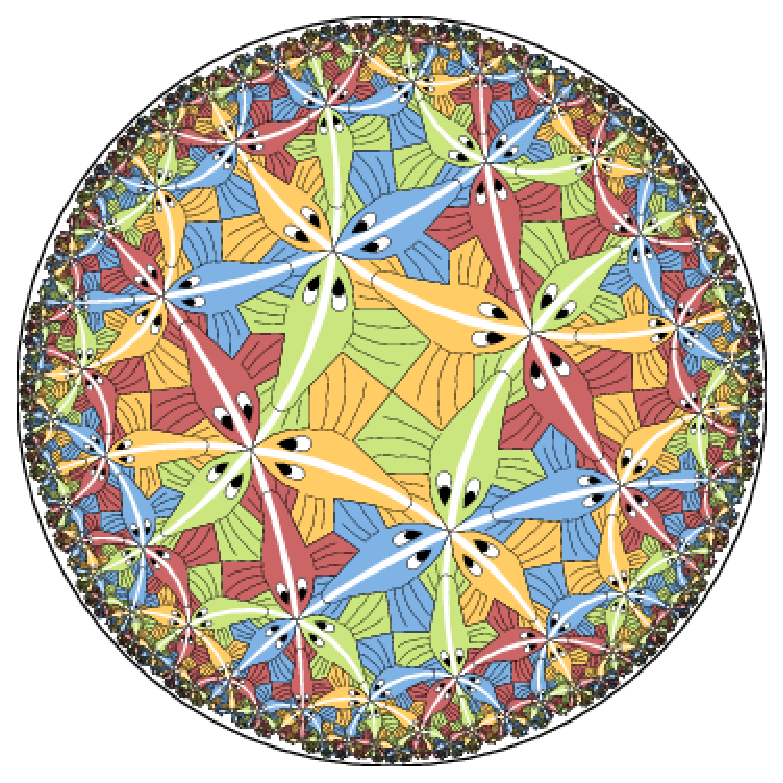
\includegraphics{circlelimit}}
\caption{A re-creation of Escher's \emph{Circle Limit III}, 
a depiction of hyperbolic geometry on the Poincar\'e disc.
Taken from \cite{transhyp}.}
\label{fig:circlelimit}
\end{figure}



\subsection{Space-Time Algebra}

\section{Extending the Conformal Model}
\subsection{Spherical Geometry}
\subsection{Hyperbolic Geometry}


All rigid-body transformation (i.e.\ rotation and translation) rotors in 
the Euclidean approach above leave $n$ invariant, i.e.\ 
$Rn\tilde{R} = n$ for all rotors $R$. They also leave $\bar{n}$ invariant. We have
already identified $n$ and $\bar{n}$ with the points at infinity and the origin 
respectively. The question arises: `What if we restrict rotors to keep other
vectors invariant?'. Since a geometry is defined by its congruence transformations,
changing those transformations will therefore reflect a different geometry.

Instead we choose to restrict the rotors such that they keep $e$
invariant. Without loss of generality, we deal with a conformal extension of
$\mathbb{R}^2$ and write down a set of four basis vectors
\begin{equation}
E_1 = e_1 \quad E_2 = e_2 \quad E_3 = e \quad E_4 = \bar{e}
\end{equation}
and thus form the rotors $R_{k\ell } = \exp\left(\frac{\alpha}{2}E_k \wedge E_\ell\right)$ with $k,\ell \in \{1,2,3,4\}$.
Applying them to $e$ via $R_{k\ell }e\tilde{R}_{k\ell } \equiv R_{k\ell }eR_{\ell k}$ we find
the bivector generators of the rotors which preserve $e$ are $\bar{e}e_1$, 
$\bar{e}e_2$ and $e_1e_2$. The latter just correspond to rotations in the
$e_1e_2$ plane and hence, the former two must be the generators of
translations.

Hence we can say that a rotor which translates the origin to the vector
$x$ must be given by
\begin{equation}
T_x = \exp\left(\frac{f(r)}{2}\bar{e}\hat{r}\right)
\end{equation}
where $r = |x|$, $\hat{r} = x/|x|$ and $f(r)$ is some function of $r$ yet to
be determined. Noting that $(\bar{e}{e_1})^2 = (\bar{e}e_2)^2 = +1$ and therefore
$(\bar{e}\hat{r})^2 = +1$ we can take the power series expansion of $T_x$ and
collect like-coefficients to obtain
\begin{equation}
T_x = \cosh\left(\frac{f(r)}{2}\right) + \bar{e}\hat{r}\sinh\left(\frac{f(r)}{2}\right)
\label{eqn:nonEuclidTrans1}
\end{equation}

The choice of the origin is only restricted in that it must differ from the 
point at infinity and must not contain components of $e_1$ or $e_2$ (to retain
isotropy). Either $n$ or $\bar{n}$ is a suitable choice but we choose
a multiple of $\bar{n}$
to retain compatibility with the Euclidean case.

Again, as with the Euclidean case, we wish to impose a normalisation condition 
on the null-vectors, 
$X = F_e(x)$, such that 
\begin{equation}
X \cdot e = -1
\end{equation}
where we use $F_e(x)$ to represent the mapping defined by the geometry
generated by the rotors which
preserve $e$. If this is to hold then the origin must in fact be $-\bar{n}$.

We can now find the representation of the general point $x$ as the translation
along $x$ of the origin. Writing $c = \cosh\left(\frac{f(r)}{2}\right)$ and
$s = \sinh\left(\frac{f(r)}{2}\right)$
\begin{eqnarray}
F_e(x) & = & T_x\,(-\bar{n})\,\tilde{T}_x \\
& = & \left[c + \bar{e}\hat{r}s\right] (-\bar{n}) \left[c - \bar{e}\hat{r}s\right] \\
&=& -c^2\bar{n} + 2sc\hat{r} + s^2n 
\end{eqnarray}
then letting $C = \cosh(f(r))$ and $S = \sinh(f(r))$ giving $c^2 = (C+1) / 2$,
$s^2 = (C-1)/2$, $sc = S/2$ and hence
\begin{eqnarray}
F_e(x) & = & \frac{1}{2}n (C-1) - \frac{1}{2}\bar{n}(C+1) + S\hat{r} \\
& = & \frac{1}{2} \left[ \, (C-1)n + 2S\hat{r} - (C+1)\bar{n} \, \right] 
% & = & \frac{1}{2} \left[ \, (\cosh(f(r))-1)n + 2\sinh(f(r))\hat{r} - (\cosh(f(r))+1)\bar{n} \, \right] 
\end{eqnarray}
As required $(F_e(x))^2 = 0$ and $F_e(x) \cdot e = -1$.

It remains to choose a sensible form for $f(r)$. We seek to choose $f(r)$ such that
the representation $F_e(x)$ is similar to our Euclidean representation $F(x)$
since this will allow us to use many of the same techniques we developed for the
Euclidean case. We can re-write our Euclidean representation 
in terms of $r$ and $\hat{r}$ as
\begin{equation}
F(x) = \frac{1}{2\lambda^2}(r^2n + 2 \lambda r\hat{r} - \lambda^2\bar{n})
\label{eqn:nonEuclidMap1}
\end{equation}

If we wish that $F_e(x)$ be similar to $F(x)$ then we have the conditions
\begin{equation}
\frac{S}{C + 1} = \frac{\sinh(f(r))}{\cosh(f(r)) + 1} = \frac{r}{\lambda}
\label{eqn:rlambda}
\end{equation}
and
\begin{equation}
\frac{C-1}{S} = \frac{\cosh(f(r)) - 1}{\sinh(f(r))} = \frac{r}{\lambda}
\label{eqn:rlambda2}
\end{equation}
so the mapping function becomes
\begin{eqnarray}
F_e(x) &=& \frac{C+1}{2\lambda^2}\ [x^2n + 2\lambda x - \lambda^2 \bar{n}] \\
&=& \frac{\cosh(f(r)) + 1}{2\lambda^2}\ [x^2n + 2\lambda x - \lambda^2 \bar{n}]
\end{eqnarray}
which has a degree of similarity to the expression for $F(x)$. Further, 
assuming $r$ and $\lambda$ are positive, we can see from equation
\ref{eqn:rlambda} that $r < \lambda$ since $\sinh(A) < 1 + \cosh(A)$
for all $A$.

Given equations \ref{eqn:rlambda} and \ref{eqn:rlambda2}, we can eliminate
$\sinh(f(r))$ to give
\begin{equation}
\frac{\cosh(f(r)) -1}{\cosh(f(r)) + 1} = \frac{r^2}{\lambda^2}
\end{equation}
and hence $\cosh(f(r)) = (\lambda^2 + r^2)/(\lambda^2 - r^2)$. Substituting
into either \ref{eqn:rlambda} or \ref{eqn:rlambda2} gives
\begin{equation}
f(r) = \sinh^{-1}\left( \frac{2\lambda r}{\lambda^2 - r^2} \right)
\end{equation}
and hence we can form the following expressions for 
$\sinh(f(r))$ and $\cosh(f(r))$
\begin{equation}
\sinh(f(r)) = \frac{2\lambda r}{\lambda^2 - r^2} \quad \mbox{ and } \quad
\cosh(f(r)) = \frac{2\lambda^2}{\lambda^2 - r^2} - 1
\end{equation}

Inserting these into equation \ref{eqn:nonEuclidMap1} gives the final form
of the non-Euclidean mapping function
\begin{equation}
F_e(x) = \frac{1}{\lambda^2 - x^2}(x^2 + 2\lambda x - \lambda^2\bar{n})
\label{eqn:nonEuclidMapping}
\end{equation}

We can also show that the form of the translation rotor given in 
\ref{eqn:nonEuclidTrans1} can be written as
\begin{equation}
T_x = \frac{1}{\sqrt{\lambda^2 - x^2}}(\lambda + \bar{e}x)
\end{equation}

By finding the metric as shown in Lasenby \emph{et al.} (2002) it can be shown
that this gives rise to the Poincar\'e disc representation of non-Euclidean
geometry (see Brannan \emph{et al.} \cite{GEOM:brannan} for a description of the 
Poincar\'e disc).

Some discussion of the relevance of $\lambda$ is worthwhile here. Notice that
in order for the translator to remain real-valued, $x^2 \le \lambda^2$. 
We can never therefore translate the origin outside of a circle radius
$\lambda$ centred upon it. The value of $\lambda$ effectively defines
a region of inaccessible space from the origin, effectively a boundary to
the geometry.

This circle corresponds directly to the unit-circle boundary in the
Poincar\'e disc representation if $\lambda = 1$ and simple dilations of
the Poincar\'e representation if $\lambda \ne 1$. To maintain compatibility
with the Poincar\'e representation, we usually set $\lambda$ to be unity.

\subsection{Space-Time Algebra}
\section{Non-Euclidean Visualisation Methods}
\subsection{NURBs}

A key requirement for visualising objects in the Poincar\'e disc
representation of hyperbolic geometry is to plot representations of
straight lines, known as $d$-lines. This chapter outlines a method 
developed to draw them using OpenGL and also presents a generalisation
of the method for drawing analogous `$d$-planes' in three-dimensional
hyperbolic geometry.


The $d$-lines on the Poincar\'e disc are circular arcs (and straight lines
for the special cases of lines through the origin). OpenGL, the graphics
library used for the implementation, has native support for a class
of curves called \emph{NURBS} (Non-uniform Rational B-Splines) 
\cite{mecg}. 

%It is
%not the r\^ole of this report to provide a complete tutorial on NURBS,
%suffice it to say that they provide a way of parametising a large class of
%curves by a set of \emph{control points} and associated \emph{weights}.

NURBS curves are specified using a set of control points, $P_i$,
weights, $w_i$ and a set of normalised basis functions $N_{i,k}$.
The curve is given by
\[
C(u) = \frac{\sum_{i=0}^n w_i P_i N_{i,k}(u)}{\sum_{i=0}^n w_i N_{i,k}(u)}
\]

The basis functions are defined recursively:
\[
N_{i,k}(u) = \frac{u - t_i}{t_{i+k} - t_i} N_{i,k-1}(u) +
  \frac{t_{i+k+1} - u}{t_{i+k+1} - t_{i+1}} N_{i+1,k-1}(u)
\]
with
\[
N_{i,0} = 
\begin{cases}
1 \mbox{ if } t_i \le u \le t_{i+1} \\ 
0 \mbox{ otherwise} 
\end{cases}
\]
and $t_i$ being the elements of the \emph{knot vector}
\[
U = \{ t_0, t_1, ... , t_m \}
\]

The relation between the number of knots, $m+1$, the degree $k$ of 
the functions $N_{i,k}$ and the number of control points, $n+1$
is given by $m = n + k + 1$ \cite{peigl, rogers}.

Clearly a large family of curves can be expressed with suitable choices
of knot vectors, weights and control points leading to great flexibility.
All NURBS curves share some common properties however which make them
useful in Computer Graphics. A NURBS curve \emph{always} stays inside the
convex hull of its control points \cite{rogers} and thus is is very easy
to compute whether the curve will be displayed at all. Further they
are tangential to the piece-wise linear interpolation of control
points and the end-points, see figure \ref{fig:samplenurb}.

\begin{figure} \centering
\scalebox{0.9}{\includegraphics{samplenurb}}
\caption{A set of control points and a typical example of an associated
NURBS curve. Note that the endpoints of the curve are tangential to
$P_0P_1$ and $P_5P_6$ and that the curve is within the convex hull
of the points (shaded).}
\label{fig:samplenurb}
\end{figure}

\subsection{Rendering $d$-lines}

To draw $d$-lines on the Poincar\'e disc, we wish to draw circular arcs
with end-points on the boundary circle and erupting normal to it.

A large number of different curves can be created with different control 
point numbers, positions and weights. Fortunately there are a number of
standard techniques to generate common curves. One such method of
drawing arcs is useful to us. We use three control
points; one at the start of the circular arc, one at the origin of the
boundary circle and one
at its end, see figure \ref{fig:nurbs}. 
The end-point weights are unity whereas the weight of the control
point at the origin is $\cos \gamma$ where $\gamma$ is the angle
$OA$ makes with $AB$\footnote{See http://www.ddt.pwp.blueyonder.co.uk/evgeny/Intro/NURBS.htm for a demonstration of this.}. 

\begin{figure} \centering
\scalebox{0.7}{\includegraphics{nurbs}}
\caption{NURBS-based rendering of $d$-lines. Here $O$ is the origin and
$A$ and $B$ are the boundary points of the line $L$.}
\label{fig:nurbs}
\end{figure}

Since NURBS are tangential to the piecewise linear interpolation of control 
points
at either end, it is clear that the curve erupts from the boundary
tangential to the lines $OA$ and $OB$. Given $O$ is the origin, and the
boundary is centred upon it, these lines are radii of the boundary
circle and so clearly are normals.

This allows us to construct a NURBS representation of any $d$-line
on the Poincar\'e disc (including diameters) and efficiently draw them
using OpenGL. 

\subsubsection{Calculating properties of $d$-lines}

The last step in drawing out $d$-lines is now finding where they intersect
the boundary disc, their \emph{boundary points}. 
Once we have these points, the drawing can be performed
via our NURBS-based method outlined above.

We can calculate approximate boundary points of $d$-lines
by forming a circle 
corresponding to the boundary and finding the 
meet of the line with this circle. This gives the null-vector
representation of the boundary points $A$ and $B$ as the
bivector $A \wedge B$ as with circle/sphere intersections and the like.
We have already shown that this bivector can be factorised into $A$ and 
$B$ via the method of projectors.
We finally need to calculate the angle $\gamma$ which is a trivial
exercise in trigonometric geometry. 

Figure
\ref{fig:hyp1} shows the rendering of $d$-lines in action.
Here we have three $d$-lines created by rotating and translating the
diameter to form a hyperbolic triangle (central dark-shaded
region). Each of these lines were reflected in the other two to form 
a set of three reflected triangles (outer light-shaded regions). This
operation could be repeated to tile the space.

\begin{figure} \centering
\scalebox{0.5}{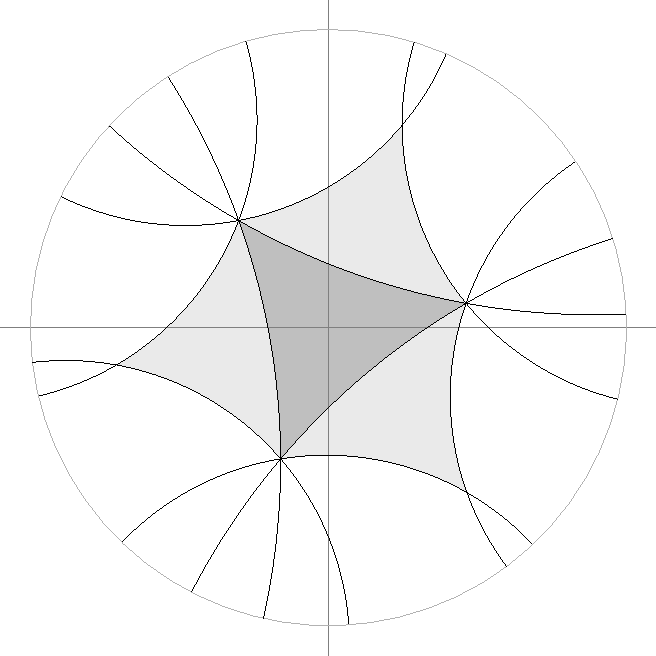
\includegraphics{hyperbolic1}}
\caption{NURBS rendering of $d$-lines in action.}
\label{fig:hyp1}
\end{figure}

\subsection{Rendering `$d$-planes'}


Drawing $d$-lines is interesting in itself but is an already solved 
problem many-times over. What is interesting is the generality the CGA
approach provides. Recalling our discussion of the development of
hyperbolic geometry in CGA, at no point did we ever assume only 
two-dimensions. We now have the intriguing opportunity to investigate
visualisation algorithms in three-dimensions.

We'll first assume that there is some analogous form to the Poincar\'e
disc representation for three-dimensions. In this case, $d$-lines can
be drawn using a similar method, this time intersecting them with a 
boundary sphere to find the two points of eruption. What would be 
more interesting is attempting to find the form for `$d$-planes'.

The method of defining planes in hyperbolic geometry is identical
to our definition in Euclidean geometry; given four points on the
$d$-plane, $\{ x_1, ..., x_4 \}$, the plane $\Phi$ is defined as
\begin{equation}
\Phi = \bigwedge_{i = 1...4} F_e(x_i)
\label{eqn:plane}
\end{equation}
Note we have incorporated the mapping into null-vectors within
the definition. Any point, $p$, which lies on the plane $\Phi$ satisfies
\[
F_e(p) \wedge \Phi = 0
\]

The drawing of $d$-planes is, however, less straight-forward. Firstly we
need to find what shape they are when represented in the Poincar\'e sphere.
Recall that
\[
F_e(x) = \frac{1}{\lambda^2 - x^2} (x^2 + 2\lambda x - \lambda^2\bar{n})
 =  \frac{2\lambda^2}{\lambda^2 - x^2} F(x)
\]
where $F(x)$ is the mapping function for Euclidean geometry. The factor
$(2\lambda^2) / (\lambda^2 - x^2)$ is always scalar for any vector
$x$ and we shall represent it as the function $s(x)$. Hence we can
re-write equation \ref{eqn:plane} as
\begin{eqnarray}
\Phi & = & \bigwedge_{i = 1...4} s(x_i)F(x_i) \\
     & = & \left[\prod_{i = 1...4} s(x_i)\right] \bigwedge_{i = 1...4} F(x_i) \\
     & = & S(x_1, x_2, x_3, x_4) \bigwedge_{i = 1...4} F(x_i) 
%%     & = & \left[\prod_{i = 1...4} s(x_i)\right] \Sigma
\end{eqnarray}

Now $\Phi$ is defined as the product of some scalar function, $S(...)$
of the defining points and the \emph{Euclidean} definition of a sphere. This
allows us to infer that, within the Poincar\'e sphere, a $d$-plane passing
through points $\{x_1, ..., x_4\}$ is represented by a sphere passing
through those same points.

\begin{figure} \centering
\scalebox{0.7}{\includegraphics{dplane}}
\caption{$d$-planes are caps of the corresponding Euclidean sphere.}
\label{fig:dplane}
\end{figure}

It has thus been found, without doing \emph{any} explicit calculations with
the metric, that
$d$-planes are represented in the Poincar\'e sphere by portions of spheres.
This neatly shows the analytical simplicity that this approach provides.
Figure \ref{fig:dplane} shows the
relation between $d$-planes and the corresponding Euclidean sphere.

%This nicely illustrates the analytical power that CGA provides us
%with. We have managed to obtain the form of a $d$-plane without
%resorting to complex extreemality calculations and, interestingly,
%without ever explicitly finding the metric. This suggests a powerful
%technique for inverstigating geometries where the geometry is well 
%known but the metric is awkward to deal with. The hyperbolic-tangent
%form for the metric in hyperbolic geometry is tedious to deal with
%analytically but we can infer important properties of the geometry
%intuitively with this approach.

We can find the meet between the associated Euclidean sphere and the
boundary sphere to give the circle of intersection. Inspecting figure
\ref{fig:dplane} we
see that this circle is the edge of the spherical
cap corresponding to the $d$-plane.

The spherical cap forming the $d$-plane can be thought of as the
intersection of the half-space containing the origin and bounded
by the plane of intersection (see figure \ref{fig:sphereplane}).
The circle of intersection is important since we wish to extract
this \emph{plane} of intersection efficiently. This is trivial
if we note that the circle is equivalent to the wedge-product of three
points on the circumference we can form the plane of the circle
by simply wedging the circle with $n$. In summary,
the plane of intersection, $P$ can be found from the $d$-plane $\Phi$ in
the following manner:
\[
P = k (\Phi \vee B) \wedge n
\]
where $B$ is the Euclidean representation of the boundary sphere
and $k$ is some scale factor.

\begin{figure} \centering
\scalebox{0.3}{\includegraphics{sphereplane}}
\caption{$d$-plane spherical cap is intersection of associated sphere and half-space
to right of plane $P$.}
\label{fig:sphereplane}
\end{figure}

Bajaj \emph{et al.} \cite{spherecap} provide a method of finding
a suitable set of control points and NURBS parameter space clipping
curve to draw spherical caps from sphere/half-space intersections.

Their approach gives a set of control points and weights that together
draw a little more than one hemisphere. Circular clipping paths in the 
parameter space are then used to form spherical caps.

This method was used to draw the spherical caps in the implementation.
\section{Guidelines for Generalising Euclidean Algorithms}
